\section{Implementation strategy}
%
The implementation was done in C and can be found in the file \verb+poisson-mpi.c+. The whole algorithm focuses on the tree steps in the previous section. As it should be able to run on supercomputers, it was necessary to use distributed memory model. This was done using MPI. To be able to do \textbf{step 1} and \textbf{step 3} with the fast sine transform, the external code \verb+fst.f+ was used. However, this code demands a problem size (number of rows) $n = 2^k$, where $k$ is some integer. It also needed to work on a whole column at a time. The way \textbf{step 1} (\textbf{step 3} is solved exactly the same way) is done with the fast sine transform is as follows
%
\begin{align}
\underline{\tilde{G}} = \underline{S}^{-1} \left( (\underline{S} \: \underline{G})^T   \right),
\end{align}
%
where $S$ and $S^{-1}$ is the fast- and inverse fast sine transform respectively. So this is done in three steps
%
\begin{align}
  \underline{G} &\leftarrow \underline{S} \: \underline{G},\\
  \label{eq:transp} 
  \underline{A} &\leftarrow \underline{G}^T,\\
  \underline{\tilde G} &\leftarrow \underline{S}^{-1} \: \underline{A}.
\end{align}
%
The second step \eqref{eq:transp} will require sending between processes as long as a column, row, or block layout is used. Therefore it is reasonable to distribute the matrices column-wise among the processes. As $n$ is a power of two, the number of internal nodes, and therefore the size of the matrices, are $m = n-1$ which is odd. When $m$ is not a multiple of the number of processes $p$, the extra columns are given to the last process. One could have distributed them more evenly among the processes, but this was tested and did not have a significant impact on the computation time as $n >> p$.

As the fast sine transform need columns, the matrices was allocated column-wise in an attempt to make good use of cache. When transposing the $\underline{G}$, it would better with a row mayor layout, but as there are only two transpose operations, but a total to 2 fast sine transforms and 2 inverse fast sine transforms, the column-mayor layout seemed the best choice. \\
%
\begin{figure}[h!]
\begin{center}
    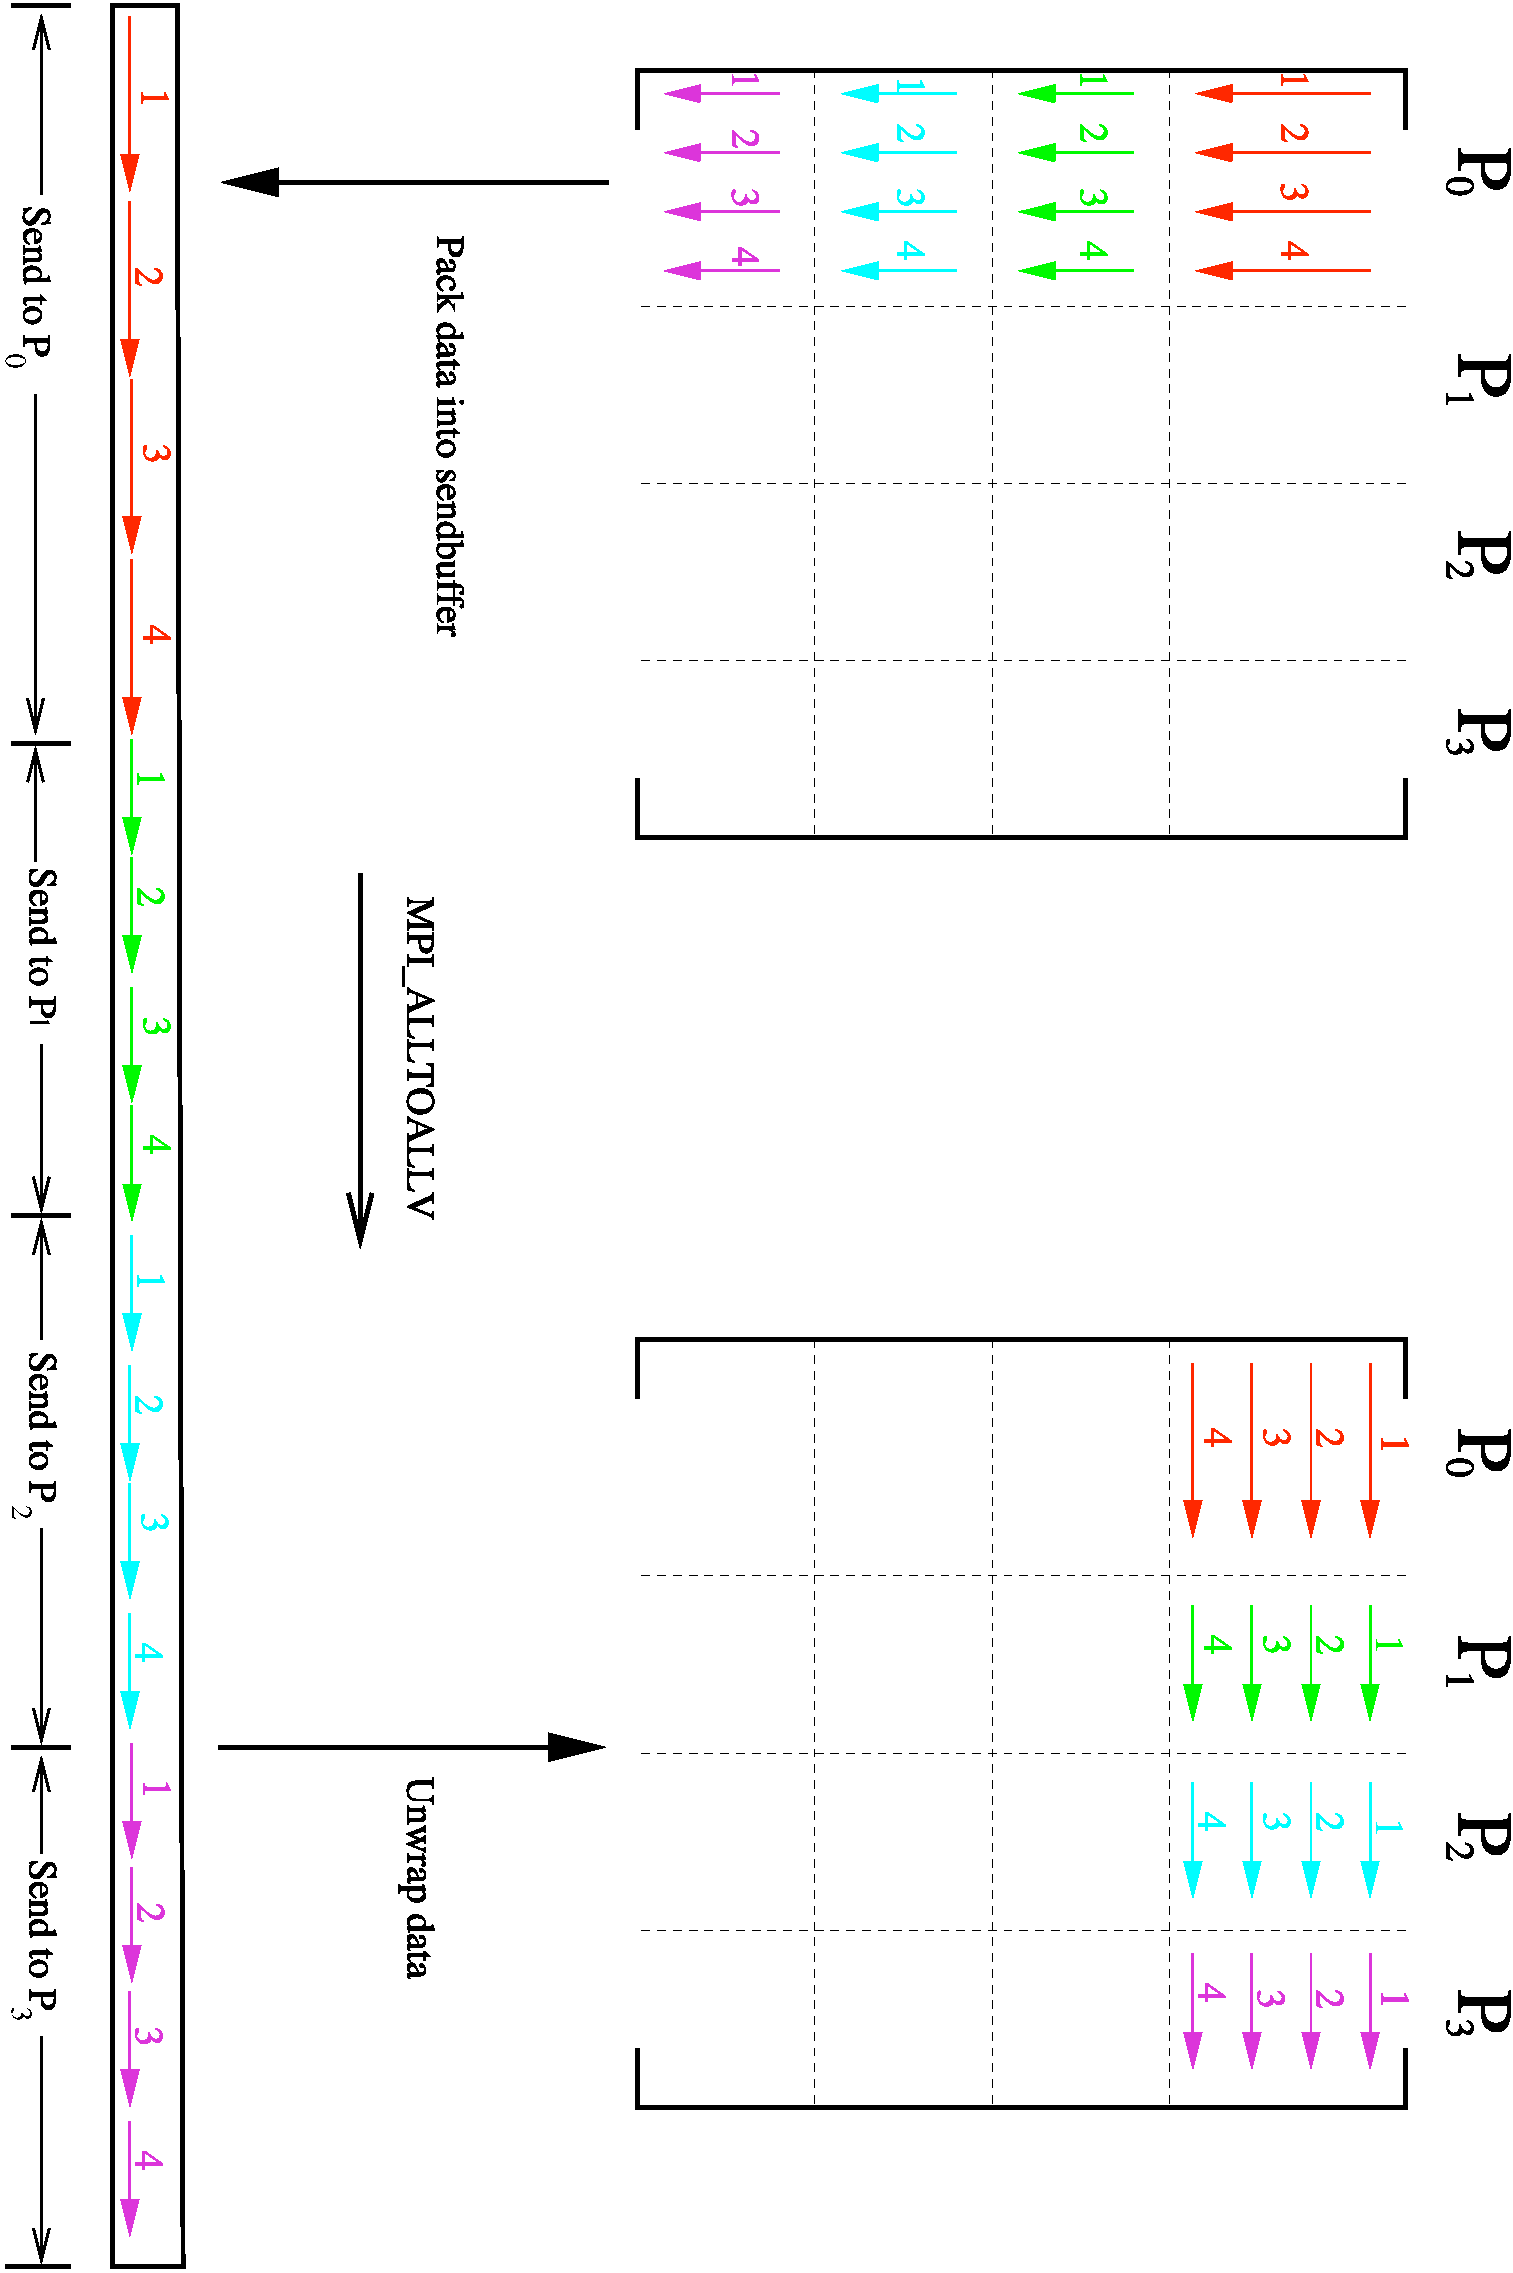
\includegraphics[angle=90,scale=0.35]{./Figures/matrix_blocktranspose.pdf}
\end{center}
\caption{The transpose operation using message passing: the packing and unpacking of data. The figure is due to Bjarte Hægland.}
\label{fig:mpisend}
\end{figure}
\\
When transposing the matrix, all the processes need to send data to each other. This is in principle done as in Figure~\ref{fig:mpisend}. However, as the matrix of each process is structured column-wise, the local matrix ($m \times r_i$ for process $i$) is first transposed locally (to $r_i \times m$). Then the data is sent to the different processes with \verb+MPI_Alltoallv+, and the data is restructured to create the transpose. \\
\\
The implementation is done so that only two matrices are needed (in addition to some vectors of length $n$). Thus \ref{eq:transp} might be a bit misleading when it comes to memory usage. With only two matrices each process use approximately $2 n^2/p$ doubles of memory, and each node use around a total of $2 n^2/nodes$. For the larges computations done in this project, $n = 2^{14} = 16384$, each node use around $4/nodes$ GB of memory.
%
\subsection{OpenMP}
\label{sub:OpenMP}
A distributed memory model is needed to run on multiple nodes. However, it hight be faster to use threads and shared memory on each machine, than dividing into MPI processes. Therefore, openMP was used to achieve this. 
All calls to the fast sine transform operates at one column at a time, therefore this was easily parallelized. A static scheduler was used, under the assumption that the fast sine transform takes a fixed amount of time for a give problem size. OpenMP was also used to crate the $\underline{G}$ matrix and doing \textbf{step 2} as they are also embarrassingly parallel. The only difficult problem to parallelize was the loops used in the transposing. However, this was achieved by using openMP for each MPI process. For many MPI processes (eg. many nodes), this will cause a lot of opening and closing of threads, but as this problem is only run on a maximum of 3 nodes, it is not considered a problem. \\
\\
As all the parallelization is pretty straight forward and the computation time of the fast sine transform only varies with $n$, the program should be well load balanced. As mentioned earlier one process gets up to $p-1$ more columns than the others. However, as $n >> p$ the program should still be well load balanced.
%
%

